% Rafael Sartori M. dos Santos, 186154
\documentclass[brazilian,a4paper,twocolumn]{article}

% Título
\title{MC920 -- Trabalho 2}
\author{Rafael Sartori M. Santos, 186154}
\date{1 de outubro de 2019}

% Configuração do documento
\setlength{\parskip}{3pt}
\usepackage[utf8]{inputenc} % tipo de documento UTF-8
\usepackage{mathtools} % permitir expressões matemáticas
\usepackage{breqn} % equações quebradas em várias linhas automaticamente
\usepackage{babel} % configuração da lingua portuguesa
\usepackage{caption} % para legenda de tabelas e figuras
\usepackage[
    pdfauthor={Rafael Sartori M. Santos},
    pdftitle={Trabalho 2 -- MC920},
    pdfproducer={LaTeX (texlive) com hyperref}
]{hyperref} % para links externos (href)
\usepackage{cleveref} % para referenciar tabelas e figuras melhor
\usepackage{indentfirst} % indentação de todo primeiro parágrafo
\usepackage{graphicx} % para adicionar imagens
\graphicspath{{../imgs_png/}, {../imgs/}} % atalho para o caminho das imagens
\usepackage{subcaption} % para imagens ficarem lado a lado
% Usamos geometry pois dá mais espaço que fullpage
%\usepackage{geometry} % alterar geometria do papel
%\geometry{a4paper,left=1.7cm,right=1.7cm,top=1cm,bottom=2.0cm} % menor margem
\usepackage{fullpage} % utilizamos uma versão com menos espaçamento nas bordas

% Início do documento
\begin{document}

\maketitle


\section{Introdução}

    Neste trabalho, temos que avaliar e comparar diferentes métodos de limiarização (locais e globais). Aplicarei cada transformação em imagens monocromáticas em formato PGM fornecidas pelo professor H. Pedrini como sugere o enunciado. O resultado analisarei quanto aos contornos dos objetos, detalhes mantidos da imagem e ruído.

    Executarei esse processamento utilizando Python com as bibliotecas padrão, \href{https://opencv.org/}{\emph{OpenCV}}, \href{https://matplotlib.org/}{\emph{Matplotlib}} e \href{https://numpy.org/}{\emph{NumPy}}.


\section{Método}

    As imagens fornecidas pelo professor foram armazenadas na pasta de entrada \texttt{imgs/} sem que fosse necessária qualquer conversão.

    Para realizar o processamento digital, as bibliotecas de Python que utilizei foram:
    \begin{itemize}
        \item \emph{OpenCV} para abrir e salvar imagens;
        \item \emph{NumPy} para aplicar transformações à imagem;
        \item \emph{Matplotlib} para produzir histogramas;
        \item Alguns módulos da padrão para interpretação da entrada (configuração de parâmetros para filtros, determinar imagem de saída, produzir informações como histogramas e relação entre pretos e brancos).
    \end{itemize}

    O código que interpreta as entradas e chama a função que corresponde ao filtro está em \texttt{main.py}. Algumas funções genéricas (aplicação de filtro, abrir e salvar imagens) estão em \texttt{util.py}. Os outros arquivos correspondem cada um a um filtro diferente de limiarização.

    Como cada filtro possui diferente número de parâmetros, utilizei o recurso de argumentos variáveis de Python (o dicionário \texttt{**kwargs}) para que consiga de forma fácil, genérica e sem depender da ordem produzir os parâmetros dos filtros com valores padrões quando não mencionados.

    Os valores que analisarei serão os padrões fornecidos no enunciado. Em alguns métodos, no entanto, irei destacar valores alternativos para possivelmente corrigir imagens poluídas.


\section{Métodos de limiarização}

    A limiarização ocorre através da comparação do ponto em que estamos considerando, $(x, y)$, com um limiar $T(x, y)$. De tal forma a produzir a imagem $g$ binária a partir de $f$ seguindo a \cref{eq:limiarizacao}.

    \begin{equation}
    \label{eq:limiarizacao}
        g(x, y) =
        \begin{cases}
            1       & \text{se $f(x, y) \geq T(x, y)$} \\
            0       & \text{caso contrário}
        \end{cases}
    \end{equation}

    Quando a limiarização é local, podemos especificar o tamanho da vizinhança quadrada $Z_{n,n}$ alterando o valor de $n$ (\texttt{--dimensao} no programa), que deve ser ímpar para que o filtro seja aplicável de forma igual numa imagem discreta. Em todos os casos, o valor padrão de $n$ foi $7$.

    \subsection{Global}

        A limiarização global é feita através de um limiar a ser aplicado em toda imagem, representado pela \cref{eq:global}.

        \begin{equation}
        \label{eq:global}
            T(x, y) = k
        \end{equation}

        O parâmetro $k$ é usado no programa para determinar o limiar global, padrozinado em $128$.

    \subsection{Bernsen}

        A limiarização local de Bernsen utiliza o máximo e mínimo dos pontos de $Z$ de acordo com a \cref{eq:bernsen}. Não possui parâmetros.

        \begin{equation}
        \label{eq:bernsen}
            T(x, y) = (Z_{min} + Z_{max}) / 2
        \end{equation}

    \subsection{Niblack}
    \label{sec:niblack}

        A limiarização local de Niblack utiliza a média $Z_{avg}$ e o desvio padrão $Z_{std}$ dos pontos de $Z$ de acordo com a \cref{eq:niblack}. Possui um parâmetro $k$ para o peso dado ao desvio padrão, padronizado em $0.8$ como no enunciado.

        \begin{equation}
        \label{eq:niblack}
            T(x, y) = Z_{avg} + k \cdot Z_{std}
        \end{equation}

    \subsection{Sauvola e Pietikäinen}
    \label{sec:sp}

        A limiarização local de Sauvola-Pietikäinen utiliza a média $Z_{avg}$ e o desvio padrão $Z_{std}$, como em \ref{sec:niblack}, através da \cref{eq:sp}, com a intenção de produzir melhores resultados sob má iluminação.

        \begin{equation}
        \label{eq:sp}
            T(x, y) = Z_{avg} \cdot \left[ 1 +  k \cdot \left( \frac{Z_{std}}{R} - 1\right) \right]
        \end{equation}

        Possui dois parâmetros: $k$ e $R$, padronizados respectivamente em $0.5$ e $128$. É abreviado no código por \texttt{SP}.

    \subsection{Phansalskar, More e Sabale}

        É uma variação de \ref{sec:sp}, porém pretende-se lidar melhor com imagens de baixo contraste. Então utiliza também a média e desvio padrão, como vemos na \cref{eq:pms}.

        \begin{multline}
        \label{eq:pms}
            T(x, y) = Z_{avg} \cdot \Biggl[ 1 +  p \cdot \exp{ \left( -q \cdot Z_{avg} \right) } \Biggr. \\ \Biggl. + k \cdot \left( \frac{Z_{std}}{R} - 1 \right) \Biggr]
        \end{multline}

        No código, é abreviado por \texttt{PMS} e utiliza todos os possíveis 4 parâmetros: $k$, $R$, $p$ e $q$, padronizados respectivamente por $0.25$, $0.5$, $2$ e $10$.

    \subsection{Contraste}

        O método local do constrate utiliza a distância relativa ao ponto mais escuro e mais claro da vizinhança: se está mais próximo de um ponto claro, é claro; se está de um ponto escuro, é escuro.

        \begin{equation}
        \label{eq:contraste}
            F =
            \begin{cases}
                0       & \text{se $\mathopen|I - Z_{max}\mathclose| \geq \mathopen|I - Z_{min}\mathclose|$} \\
                1       & \text{caso contrário}
            \end{cases}
        \end{equation}

        O ponto final $F = g(x, y)$ da imagem pode ser expresso pela \cref{eq:contraste} onde $I$ é o ponto inicial da imagem $f(x, y)$. Não requer qualquer parâmetro.

    \subsection{Média e mediana locais}
    \label{sec:media-mediana-locais}

        Consideramos a média ou a mediana dos pontos da vizinhança. Sendo esse valor o limiar $T(x, y)$, basta comparamos com o ponto em que estamos $f(x, y)$ como em \cref{eq:limiarizacao}. Também não requerem qualquer parâmetro.

    \subsection{Média e mediana globais}

        Consideramos a média ou a mediana de todos os pontos como limiar, como em \ref{sec:media-mediana-locais} considerando a vizinhança como a imagem completa.


\section{Resultados obtidos e análise}

    A avaliação dos resultados mostrou-se desafiadora: com o bem diverso conjunto de imagens de entrada, é possível notar após análise superficial que produzir um resultado satisfatório com apenas um método ``faz-tudo'' em todos os casos não foi possível. Podemos, no entanto, destacar em que partes cada método desempenha melhor e tentar explicar os motivos para isso.

    A abordagem que tomei, então, foi por agrupamento de imagens de entrada (ao invés de agrupar por método), sintetizando ao final um resumo do que os métodos foram capazes. Nesse rumo, poderemos ter uma visão geral das condições e implicar as características do método.

    \subsection{\texttt{Baboon}}

        \begin{figure}
            \centering
            \begin{subfigure}{0.30\textwidth}
                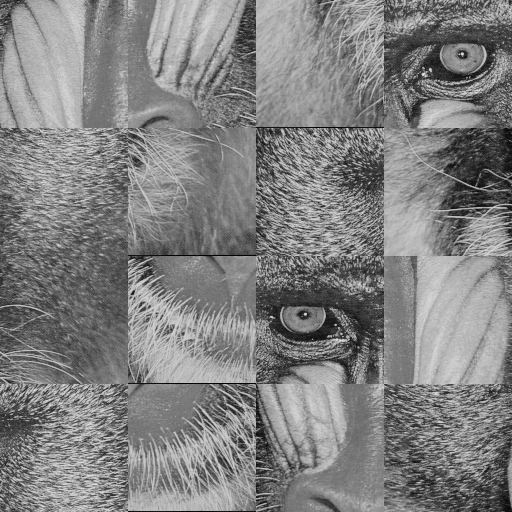
\includegraphics[width=\textwidth,keepaspectratio]{baboon}
                \caption{Imagem original \texttt{baboon}}
                \label{fig:baboon}
            \end{subfigure}
            \begin{subfigure}{0.5\textwidth}
                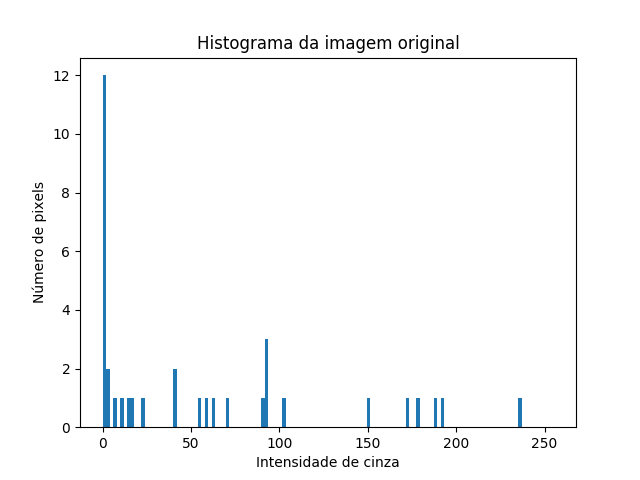
\includegraphics[width=\textwidth,keepaspectratio]{baboon-histograma_in}
                \caption{Histograma da imagem original}
                \label{fig:baboon-histograma}
            \end{subfigure}

            \caption{Características da imagem original}
        \end{figure}

        Podemos notar na \cref{fig:baboon} que há diversos detalhes finos (como os fios da pelagem, as linhas do nariz e olho). A imagem é em maioria muito nítida e possui bom contraste (\cref{fig:baboon-histograma}).

        \begin{figure}
            \centering
            \begin{subfigure}{0.23\textwidth}
                \includegraphics[width=\textwidth,keepaspectratio]{baboon-final-global}
                \caption{Método global}
                \label{fig:baboon-global}
            \end{subfigure}
            \begin{subfigure}{0.23\textwidth}
                \includegraphics[width=\textwidth,keepaspectratio]{baboon-final-bernsen}
                \caption{Método Bernsen}
                \label{fig:baboon-bernsen}
            \end{subfigure}
            \begin{subfigure}{0.23\textwidth}
                \includegraphics[width=\textwidth,keepaspectratio]{baboon-final-niblack}
                \caption{Método Niblack}
                \label{fig:baboon-niblack}
            \end{subfigure}
            \begin{subfigure}{0.23\textwidth}
                \includegraphics[width=\textwidth,keepaspectratio]{baboon-final-sp}
                \caption{Método de Sauvola e Pietikäinen}
                \label{fig:baboon-sp}
            \end{subfigure}
            \begin{subfigure}{0.23\textwidth}
                \includegraphics[width=\textwidth,keepaspectratio]{baboon-final-pms}
                \caption{Método PMS}
                \label{fig:baboon-pms}
            \end{subfigure}
            \begin{subfigure}{0.23\textwidth}
                \includegraphics[width=\textwidth,keepaspectratio]{baboon-final-contraste}
                \caption{Método do contraste}
                \label{fig:baboon-contraste}
            \end{subfigure}
            \begin{subfigure}{0.23\textwidth}
                \includegraphics[width=\textwidth,keepaspectratio]{baboon-final-media-local}
                \caption{Método da média local}
                \label{fig:baboon-media}
            \end{subfigure}
            \begin{subfigure}{0.23\textwidth}
                \includegraphics[width=\textwidth,keepaspectratio]{baboon-final-mediana-local}
                \caption{Método da mediana local}
                \label{fig:baboon-mediana}
            \end{subfigure}

            \caption{Comparativo entre diversos métodos de limiarização}
            \label{fig:baboon-limiarizacao}
        \end{figure}

        Os principais métodos que favorecem as características da imagem, de forma a destacar as linhas e detalhes sem grandes perdas visuais, são os locais: contraste (\cref{fig:baboon-contraste}), Bernsen (\cref{fig:baboon-bernsen}) e média (\cref{fig:baboon-media}).

        Nesses métodos, podemos notar um destaque claro às principais linhas da imagem. Com métodos de realce, talvez seja possível isolar uma imagem ``caricatural'' do babuíno e identificar formatos parecidos por comparação.

        Já em Niblack (\cref{fig:baboon-niblack}) e mediana (\cref{fig:baboon-mediana}), há uma proximidade aos mencionados anteriormente, mas as linhas que são destacadas pelos outros nesses métodos não são tão contínuas ou fortes. Isso tornaria a análise proposta (isolar detalhes através de processamento de imagem) mais difícil.

        Nos outros métodos locais SP (\cref{fig:baboon-sp}) e PMS (\cref{fig:baboon-pms}), há muitas perdas pelo nível de brilho ou contraste inadequados à transformação aplicada. Já nos métodos globais (global, \cref{fig:baboon-global}, média e mediana -- cujas imagens não são mostradas por serem muito próximas às do limiar global).

    \subsection{\texttt{Fiducial}}

        \begin{figure}
            \centering
            \begin{subfigure}{0.30\textwidth}
                \includegraphics[width=\textwidth,keepaspectratio]{fiducial}
                \caption{Imagem original \texttt{fiducial}}
                \label{fig:fiducial}
            \end{subfigure}
            \begin{subfigure}{0.5\textwidth}
                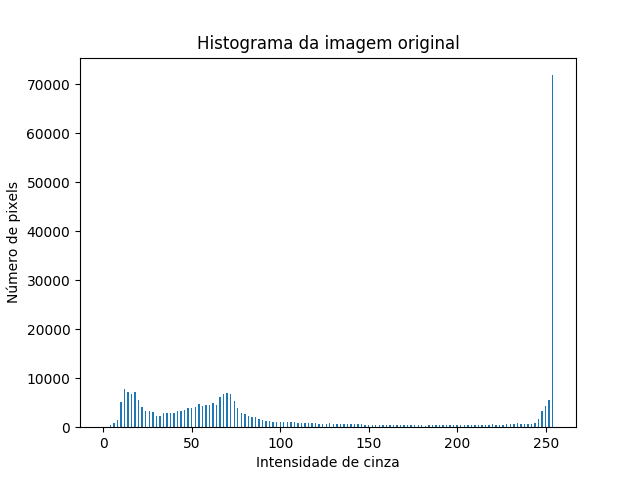
\includegraphics[width=\textwidth,keepaspectratio]{fiducial-histograma_in}
                \caption{Histograma da imagem original}
                \label{fig:fiducial-histograma}
            \end{subfigure}

            \caption{Características da imagem original}
        \end{figure}

        Podemos notar na \cref{fig:baboon} que há diversos detalhes finos (como os fios da pelagem, as linhas do nariz e olho). A imagem é em maioria muito nítida e possui bom contraste (\cref{fig:baboon-histograma}).

        \begin{figure}
            \centering
            \begin{subfigure}{0.23\textwidth}
                \includegraphics[width=\textwidth,keepaspectratio]{fiducial-final-global}
                \caption{Método global}
                \label{fig:fiducial-global}
            \end{subfigure}
            \begin{subfigure}{0.23\textwidth}
                \includegraphics[width=\textwidth,keepaspectratio]{fiducial-final-bernsen}
                \caption{Método Bernsen}
                \label{fig:fiducial-bernsen}
            \end{subfigure}
            \begin{subfigure}{0.23\textwidth}
                \includegraphics[width=\textwidth,keepaspectratio]{fiducial-final-niblack}
                \caption{Método Niblack}
                \label{fig:fiducial-niblack}
            \end{subfigure}
            \begin{subfigure}{0.23\textwidth}
                \includegraphics[width=\textwidth,keepaspectratio]{fiducial-final-sp}
                \caption{Método de Sauvola e Pietikäinen}
                \label{fig:fiducial-sp}
            \end{subfigure}
            \begin{subfigure}{0.23\textwidth}
                \includegraphics[width=\textwidth,keepaspectratio]{fiducial-final-pms}
                \caption{Método PMS}
                \label{fig:fiducial-pms}
            \end{subfigure}
            \begin{subfigure}{0.23\textwidth}
                \includegraphics[width=\textwidth,keepaspectratio]{fiducial-final-contraste}
                \caption{Método do contraste}
                \label{fig:fiducial-contraste}
            \end{subfigure}
            \begin{subfigure}{0.23\textwidth}
                \includegraphics[width=\textwidth,keepaspectratio]{fiducial-final-media-local}
                \caption{Método da média local}
                \label{fig:fiducial-media}
            \end{subfigure}
            \begin{subfigure}{0.23\textwidth}
                \includegraphics[width=\textwidth,keepaspectratio]{fiducial-final-mediana-local}
                \caption{Método da mediana local}
                \label{fig:fiducial-mediana}
            \end{subfigure}

            \caption{Comparativo entre diversos métodos de limiarização}
            \label{fig:fiducial-limiarizacao}
        \end{figure}

        Os principais métodos que favorecem as características da imagem, de forma a destacar as linhas e detalhes sem grandes perdas visuais, são os locais: contraste (\cref{fig:baboon-contraste}), Bernsen (\cref{fig:baboon-bernsen}) e média (\cref{fig:baboon-media}).

        Nesses métodos, podemos notar um destaque claro às principais linhas da imagem. Com métodos de realce, talvez seja possível isolar uma imagem ``caricatural'' do babuíno e identificar formatos parecidos por comparação.

        Já em Niblack (\cref{fig:baboon-niblack}) e mediana (\cref{fig:baboon-mediana}), há uma proximidade aos mencionados anteriormente, mas as linhas que são destacadas pelos outros nesses métodos não são tão contínuas ou fortes. Isso tornaria a análise proposta (isolar detalhes através de processamento de imagem) mais difícil.

        Nos outros métodos locais SP (\cref{fig:baboon-sp}) e PMS (\cref{fig:baboon-pms}), há muitas perdas pelo nível de brilho ou contraste inadequados à transformação aplicada. Já nos métodos globais (global, \cref{fig:baboon-global}, média e mediana -- cujas imagens não são mostradas por serem muito próximas às do limiar global).

\section{Conclusão}

    a

\end{document}
